% arara: indent: {overwrite: yes}
% options:
% thesis=B bachelor's thesis
% thesis=M master's thesis
% czech thesis in Czech language
% slovak thesis in Slovak language
% english thesis in English language
% hidelinks remove colour boxes around hyperlinks

\documentclass[thesis=B,czech]{resources/FITthesis}[2012/06/26]

\usepackage[utf8]{inputenc} % LaTeX source encoded as UTF-8

\usepackage{graphicx} %graphics files inclusion
% \usepackage{amsmath} %advanced maths
% \usepackage{amssymb} %additional math symbols

\usepackage{dirtree} %directory tree visualisation

% % list of acronyms
% \usepackage[acronym,nonumberlist,toc,numberedsection=autolabel]{glossaries}
% \iflanguage{czech}{\renewcommand*{\acronymname}{Seznam pou{\v z}it{\' y}ch zkratek}}{}
% \makeglossaries

\newcommand{\tg}{\mathop{\mathrm{tg}}} %cesky tangens
\newcommand{\cotg}{\mathop{\mathrm{cotg}}} %cesky cotangens

% % % % % % % % % % % % % % % % % % % % % % % % % % % % % % 
% ODTUD DAL VSE ZMENTE
% % % % % % % % % % % % % % % % % % % % % % % % % % % % % % 

\department{Katedra \ldots (Softwarové inženýrství)}
\title{	MobChar - desktop application for Game master in Dračí doupě}
\authorGN{Jan} %(křestní) jméno (jména) autora
\authorFN{Horáček} %příjmení autora
\authorWithDegrees{Jan Horáček} %jméno autora včetně současných akademických titulů
\supervisor{Ing. Zdeněk Rybola}
\acknowledgements{Poděkování}

\abstractCS{Cílem této práce je usnadnění hráčům Dračího doupěte a~zejména Pánu jeskyně usnadnit vytváření dobrodružství, postav a~předmětů pomocí jednoduché desktopové aplikace. Hlavní výhody aplikace jsou, možnost exportování dobrodružství pro mobilní aplikaci MobChar pro Pána jeskyně nebo exportování do přehledného pdf vhodné pro tisk a hraní Dračího doupěte bez mobilů a jiných zařízení. V práci jsem vytvořil aplikaci, ve které můžete pomocí grafického rozhraní vytvářet mapy dobrodružství propojené s~příšerami a předměty, které se dají na mapě najít. Veškeré výtvory se ukládají pro případné další použití. Můžete si vytvářet sbírku příšer a předmětů, které můžete i~sdílet s~ostatními Pány jeskyně a tak se nechat inspirovat ostatními.  Hlavní přínos této aplikace bude pro hráče Dračího doupěte, kteří by rádi využili moderní technologie pro tvorbu svého dobrodružství. Někteří hráči jistě ocení možnost sdílení dobrodružství s ostatními nadšenci anebo naopak se rádi nechají inspirovat ostatními hráči. Pomocí databáze již dříve vytvořených příšer a předmětů bude velice snadné vytvářet nové a ještě zábavnější dobrodružství.}

\abstractEN{Sem doplňte ekvivalent abstraktu Vaší práce v~angličtině.}

\placeForDeclarationOfAuthenticity{V~Praze}
\declarationOfAuthenticityOption{4} %volba Prohlášení (číslo 1-6)

\keywordsCS{desktopová aplikace, hra na hrdiny, rozšíření, herní scéna, MobChar, Dračí doupě, tvorba dobrodružství, Python, SQLite, XML}

\keywordsEN{desktop application, heroes games, extension, desktop games, MobChar, Dračí doupě, story creation, Python, SQLite, XML}

\begin{document}

% \newacronym{CVUT}{{\v C}VUT}{{\v C}esk{\' e} vysok{\' e} u{\v c}en{\' i} technick{\' e} v Praze}
% \newacronym{FIT}{FIT}{Fakulta informa{\v c}n{\' i}ch technologi{\' i}}

\begin{introduction}
Dračí doupě je populární hra na hrdiny, která vznikla jako česká verze hry Dungeons~\&~dragons. V~České Republice si získala velkou oblibu zvláště mezi hráči stolních her a počítačových RPG her.\\

Hráči hrají za své hrdiny, které si na začátku dobrodružství vytvořili, putují světem a zažívají 			rozličná dobrodružství, která pro ně pán jeskyně připraví. Každý hráč si může vybrat z~rozličného 			výběru 	ras, které se ve světě vyskytují a zvolit si, jakému povolání se bude věnovat. Ale ať si 			vybere mocného orkského válečníka, rychlého a úskočného hobitího zloděje nebo moudrého a mocného 			elfského válečníka, budou ho čekat složitá rozhodnutí, která určí, jakým směrem se dobrodružství 			bude ubírat dále. \\

Dračí doupě se lehce lišší od klasických stolních her, kde plán hry nebo dobrodružství máte jeden a 		toho se musíte držet. Zde celé dobrodružství vymýšlí další hráč, takzvaný pán jeskyně, který při hře 	celé dobrodružství řídí a popisuje hrdinům. Veškeré rozhodnutí, které neučiní samotní hráči rozhodne 	pán jeskyně. Příprava propracovaných a zábavných dobrodružství je velice složitá a zabere mnoho 			hodin času. Je zapotřebí vytvořit přehledné poznámky a mapy, které při hře umožní všem hráčům dobře 		pochopit situaci a oblast, ve které se právě nachází. Cílem této bakalářské práce, je tento proces 			usnadnit a zkrátit dobu přípravy, aby se pán jeskyně mohl věnovat převážně hraní s ostatními 				spoluhráči. \\

Aplikace vzniká souběžně s~mobilní aplikací MobChar pro pány jeskyně, ve které si bude možné veškeré 	informace o~dobrodružství přehledně zobrazit a prezentovat hráčům. V~balíčku aplikací již existuje 			mobilní aplikace MobChar pro hráče, která slouží pro zaznamenávání osobního deníku hráče \\


\section*{Struktura práce}
V první kapitole je popsána analýza problematiky. Popisuji zde pravidla Dračího doupěte a pravidla 			vytváření dobrodružství. Důležitá část je také analýza již existujících aplikací, ať už se jedná o 			aplikace, které by tato aplikace měla nahradit a nebo aplikace MobChar, se kterými bude DeskChar			umět komunikovat.

Na základě analýzy je v druhé kapitole popsán návrh a architektura aplikace. Jednotlivé vrstvy architektury jsou popsány do detailu a popsána komunikace mezi nimi.

Ve třetí kapitole se věnuji implementaci a testování celé aplikace a jejich jednotlivých částí.


\end{introduction}

\chapter{Úvod do problematiky}




	\section{Cíl práce}
Cílem této práce je vytvořit desktopovou aplikaci, které rozšíří již existují balíček mobilních aplikací MobChar o nové funkcionality. Hlavním účelem aplikace bude vytváření dobrodružství pro Dračí doupě. Jednou z hlavních funkcionalit je tvorba xml souborů, se kterými umí pracovat mobilní aplikace MobChar.
	\section{Dračí doupě}


\chapter{Současný stav}
	\section{Projekt MobChar}
Aplikace MobChar vznikla jako samostatná aplikace, která měla sloužit jako osobní deník hráče pro hru Dračí doupě. Postupem času se rozšiřovala a měnila základní struktura. Nynější stav již umožňuje vytváření rozšíření pro další hry na hrdiny jako jsou například Dungeons~\&~Dragons. V této chvíli jsou již plně funkční rozšíření pro Dračí doupě a Dungeons~\&~Dragons a vznikají další.\\
\\
V rámci aplikace MobChar vzniká další rozšíření, ne však pro osobní deník hráče, ale pro pána jeskyně. Jednoduchá aplikace, ve které budou k dispozici údaje o všech hráčích a údaje od právě probíhajícím dobrodružství. Protože tvorba dobrodružství je poměrně náročná činnost, která vyžaduje napsání mnoho textu, připravení velkého množství šablon a další, bylo by velice nepraktické toto dobrodružství vytvářet na mobilním zařízení. Proto vzniká desktopová aplikace DeskChar, jejíž hlavním cílem bude vytváření dobrodružství a šablon pro mobilní aplikace.

	\section{Existující aplikace}
Díky rozsáhlé komunitě okolo her na hrdiny jako jsou Dračí doupě a Dungeons~\&~Dragons vzniklo již mnoho aplikací, které mají hraní či přípravu dobrodružství usnadnit. Můžeme najít desítky různých editorů map, které jsou více či méně povedené a propracované. Mezi nejzajímavější bych asi zařadil Dungeon Painter Studio, který se převážně zaměřuje na tvorbu rozsáhlých map nebo například Donjon, který se zaměřuje na generování náhodných map a další objektů jako jsou například obchody,truhly, počasí a další. Všechny tyto aplikace vám vygenerují PDF soubor, který si můžete následně vytisknout a vzít sebou na herní sezení. Žádná z těchto aplikací nenabízí mobilní prohlížeč dobrodružství, nebo export do nějakého formátu, který by se dal na mobilních zařízení jednoduše prohlížet. Přeci jenom PDF soubor formátu A4 s mnoho údaji, není příliš přehledný, obzvlášť na malých obrazovkách. \\
\\
\textbf{Dungeon Painter Studion} je aplikace, která se zaměřuje na tvorbu map a následné generování PDF souborů. Existuje online verze, která je zdarma, která však nenabízí veškeré funkcionality plné verze. Ale i v této zjednodušené verzi dokážete vytvořit velmi propracované mapy. Plná verze je již desktopová aplikace, která je placená (stojí  přibližně 400 korun). Je možné zde vytvořit opravdu krásná a poutavá dobrodružství včetně stínování, světelných efektů a mnoho dalšího. Podle mého názoru, je však až zbytečně složitý a pro větší pánů jeskyně, příliš zdlouhavý. Vytvoření jedné mapy zabere opravdu hodně času a ve většině případů takto propracované mapy nejsou pro hraní důležité. Bohužel v základní verzi není možné s mapou propojit předměty a příšery z dobrodružství, což považuji za jednu z nejdůležitějších funkcionalit. \\
\\
\textbf{Donjon} je online aplikace, která se zaměřuje na generování náhodných lokací. Můžeme si zde navolit základní nastavení jako je velikost mapy, velikost místností a další. Finální verzi mapy již upravit však nemůžeme. K mapě dostaneme popis jednotlivých místností v poměrně nepřehledné tabulce. Tento formát bez dodatečných úprav v obrázkovém editoru nelze rozumě vytisknout. Aplikace nabízí generování další prvků, jako například poklady, obchody a další, bohužel však tyto vygenerované prvky se jíž nedají propojit s vygenerovanou mapou. 









\chapter{Analýza}
	\section{Požadavky}



Sběr požadavků je jedna z~prvních činností, které se musí provést na začátku analýzy projektu. Je zapotřebí sepsat veškeré funkční a nefunkční požadavky, na základě kterých bude vznikat návrh a výsledný program. Na základě požadavků se dají vytvořit první odhady na rozsah projektu a~na jeho cenu. Tento odhad je velice nepřesný, ale zákazníci vyžadují předběžnou cenu, již na základě jejich požadavků na program. 
	
\subsection{Funkční požadavky}
Funkční požadavky jsou rozděleny do dvou částí, funkcionalita pro hráče a funkcionalita pro pána jeskyně. Tyto sekce jsou rozdělené, protože popisují stejný program, ale z pohledu jiného uživatele.
\subsubsection{Funkcionalita pro hráče}
Funkční požadavky, které program bude poskytovat zejména pro hráče pro práci se šablonami.\\
\\
\textbf{Tvorba a editace šablon pro MobChar:} program bude umožňovat vytvářet nové šablony pro mobilní aplikaci MobChar. Bude také umožňovat editovat stávající šablony. Jednotlivé šablony lze přehledně uspořádat do stromové struktury.\\
\\
Šablony se kterými bude možné pracovat:
				\begin{itemize}
					\item Kouzla
					\item Předměty
					\item Schopnosti
					\item Efekty
				\end{itemize}
\textbf{Export šablon pro mobilní aplikaci MobChar:} program bude umožňovat jednoduchý a hromadný export vybraných šablon pro mobilní aplikaci MobChar ve formátu xml.\\
\\
\textbf{Import šablon z~mobilní aplikace MobChar:} program bude umožňovat import xml šablon, které se dají vytvořit v~mobilní aplikaci MobChar. Šablony se přidají do databáze a následně je bude možné editovat.\\
\\
\textbf{Ukládání šablon do souboru:} program bude umožňovat ukládat veškeré vytvoření šablony do společného xml souboru, který bude možné opět do programu načíst a nahrát veškeré šablony. Soubor bude sloužit pro jednoduché ukládání práce a sdílení šablon.

\subsubsection{Funkcionalita pro pána jeskyně}
Funkční požadavky, které program bude poskytovat zejména pro pána jeskyně pro vytváření nových dobrodružství.
\textbf{Tvorba a editace dobrodružství:} program bude umožňovat vytváření nových a editaci stávajících dobrodružství. K dobrodružství se dají přiřadit veškeré potřebné objekty, které se v aplikaci dají vytvořit. Celé dobrodružství lze členit do přehledné stromové struktury.\\
\\
\textbf{Tvorba a editace mapy pro dobrodružství:} Program bude umožňovat vytvářet a~editovat mapy pro dobrodružství. Mapa půjde vytvářet ve třech různých módech
\begin{itemize}
\item Základní mód - k dispozici budou pouze jednoduché prvky a~kreslící nástroj pro čáry
\item Grafický mód - mapa se bude skládat z~jednotlivých grafických dílků
\item Obrázkový mód - jako podklad mapy bude sloužit nahraný obrázek, který bude doplněn o jednoduché objekty
\end{itemize}
Na mapu půjdou umisťovat odkazy na vytvoření postavy, příšery, předměty a~další mapové prvky. Mapy půjdou sdružovat do stromové struktury pro větší přehlednost\\
\\
\textbf{Tvorba a~editace příšer pro dobrodružství:} program bude umožňovat vytváření nových a~editaci již existujících příšer pro dobrodružství. Příšery půjdou seskupovat do stromové struktury pro větší přehlednost.\\
\\
\textbf{Tvorba a~editace postav pro dobrodružství:} program bude umožňovat vytváření nových postav a editaci již existujících. Postavy půjdou seskupovat do stromové struktury pro větší přehlednost.\\
\\
\textbf{Exportování dobrodružství pro mobilní aplikaci MobChar:} celé dobrodružství půjde exportovat ve formátu xml se strukturou, která podporuje mobilní aplikace MobChar pro pána jeskyně.\\
\\
\textbf{Importování a~exportování dobrodružství pro sdílení:} celé dobrodružství včetně všech přiřazených objektů půjde exportovat do jednoho xml souboru, který následně bude možné do aplikace znovu nahrát. Soubor bude sloužit pro ukládání práce a~případné sdílení s~ostatními pány jeskyně.\\
\\
\textbf{Export dobrodružství pro tisk:} Aplikace bude umožňovat exportování celého dobrodružství do přehledného formátu, který je vhodný pro tisk. 
\subsection{Nefunkční požadavky}

\textbf{Podpora operačních systémů Windows a Linux:} program půjde spustit pod operačnímy systémy Windows a Linux. U operačního systému Windows budou podporovány všechny verze, které jsou novější než Windows XP. Program bude spustitelný pomocí exe souboru. U operačního systému Linux budou podporovány standardní linuxové distribuce. Program bude spustitelný pomocí bash souboru.\\
\\
\textbf{Jazyková podpora} program bude umožňovat přepínání jazyků a případnou lokalizaci pro další jazyky. V základu bude podporován český jazyk a anglický jazyk.



	\section{Případy užití}
Případy užití popisují jednotlivé činnosti, které uživatel provádí, při práci s~aplikací. Diagram byl rozdělen na tři hlavní části pro větší přehlednost.
\subsection{Práce se šablonami}
\begin{figure}\centering
	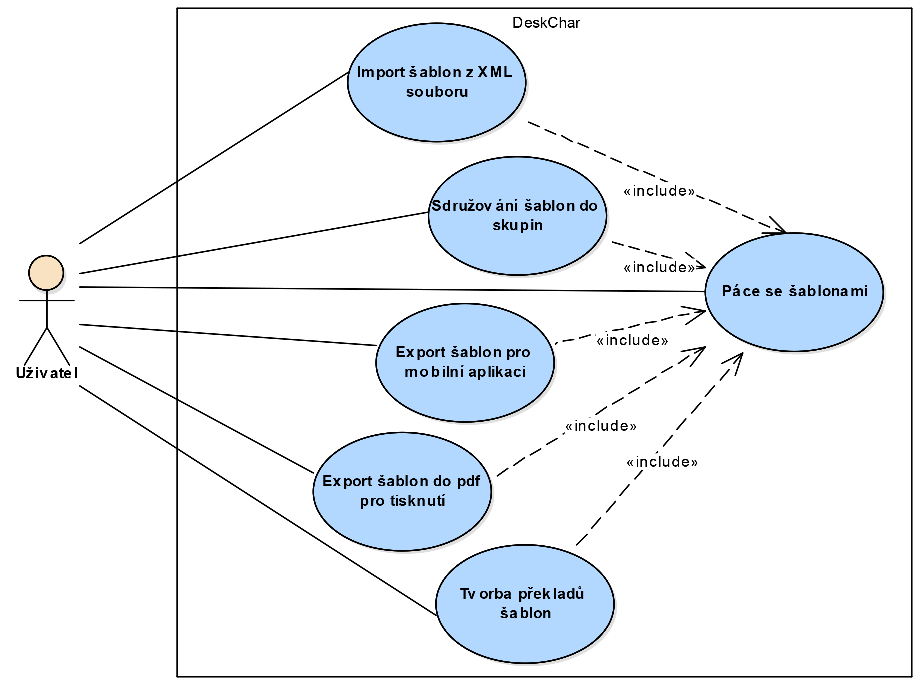
\includegraphics[width=0.8\textwidth]{images/usecase_sablony.pdf}
	\caption[Případy užití pro šablony]{Případy užití pro práci se šablonami}\label{fig:uc_sablony}
\end{figure}

Případ užití týkající se práci se šablonami namodelovaný na obrázku \ref{fig:uc_sablony} se týká veškeré práce se šablonami. Dobrodružství a postavy jsou složené z jednotlivých šablon, které se dají využít i samostatně. Nakonec i dobrodružství a postava mají formát šablony, které v sobě obsahují další šablony.\\
\\
\textbf{Vytváření a editace šablon:} uživatel si bude moci vytvořit nové šablony nebo editovat stávající. Veškeré parametry, které je možné do šablony zapsat, lze jednoduše upravovat v přehledném formuláři. Uživatel si může vytvořit libovolný počet šablon, které se na základě návazností sdružují na větších celků (dobrodružství, postava).\\
\\
\textbf{Import šablon z XML souboru:} program bude umožňovat import šablon ze strukturovaných xml souborů, které vytváří mobilní aplikace MobChar a také samotný program. Importované šablony se přidají do databáze a lze s nimi následně provádět stejné činnosti jako s nově vytvořenými. Import je možný buď hromadný, který se pokusí ze souboru dostat veškeré dostupné informace a přidat je do aplikace do příslušná místa, nebo lokální import, který ze souboru vytáhne pouze šablony o daném typu.\\
\\
\textbf{Sdružování šablon do skupin:} veškeré šablony půjde rozřazovat do stromové struktury pro větší přehlednost a jednoduší práci s nimi. Pomocí vytváření složek a jednoduchého drag and drop systému bude rozřazování velice jednoduché a intuitivní. Díky rozřazení do složek je následná práce se šablonami velice usnadněná, ať už se jedná o export nebo přiřazování do rodičovských šablon.\\
\\
\textbf{Export šablon:} veškeré vytvořené šablony lze z aplikace exportovat. K dispozici jsou různé druhy exportu. První možnost je export pro mobilní aplikace MobChar. Aplikace vytvoří strukturované XML soubory, které odpovídají formátu, který používá mobilní aplikace MobChar. Další možností exportu je PDF formát, který slouží pro tisknutí šablon do přehledného almanachu, který umožní využít šablony i hráčům, kteří mobilní aplikaci nemají nebo ji nechtějí použít. Poslední možnost exportu, je klasické uložení celého stavu šablon do jednoho xml souboru, který bude využívat stejnou strukturu šablon. \\
\\
\textbf{Tvorba překladů šablon:} ke každé šabloně vytvořené nebo importované do aplikace lze vytvořit neomezený počet překladů. Překlady se vytváří v rámci jedné šablony, pomocí přehledného přepínaní mezi jazyky. Veškeré hodnoty, pro které překlad nemá smysl (číselné hodnoty, povolání, atd.) budou synchronizování napříč všemi jazyky.\\
\\

	\section{Business procesy}
Business proces (někdy též nazývaný podnikový nebo obchodní proces) je tok práce nebo činnosti. Dají se zaznamenávat pomocí textu nebo přehledných modelů. Modely business procesů se snaží přehledně do diagramu zanést jednotlivé procesy, které bude uživatel s danou aplikací nebo doménou provádět. Já jsem zvolil UML diagram aktivit pro zachycení business procesů v mé práci.
\subsection{Vytváření šablon} \label{sec:vytvareni_sablon}
\begin{figure}\centering
	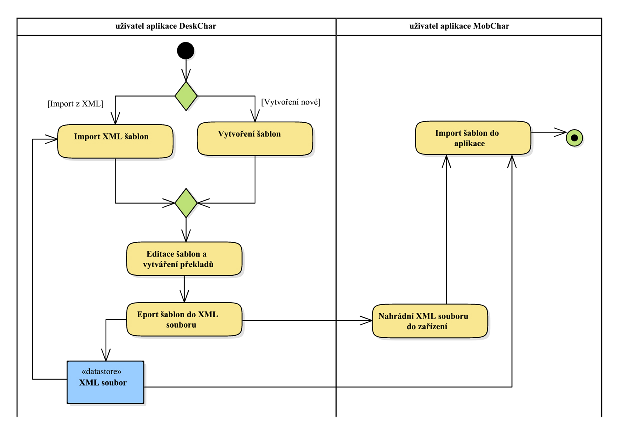
\includegraphics[width=0.8\textwidth]{images/bussiness_sablony}
	\caption[Business proces vytváření šablon]{Model bussines procesů vytváření šablon}\label{fig:bp_sablony}
\end{figure}
Diagram \ref{fig:bp_sablony} popisuje základní proces práce se šablonami. Proces popisuje vytvoření šablon a~následné nahrání do mobilní aplikace. Šablony vytvoříme v~programu nebo případně importujeme z~xml souboru vytvořeném buď aplikací nebo například aplikací MobChar. Samozřejmě import a~vytvoření nových šablon můžeme kombinovat. Při tomto procesu nevzniká pouze jedna šablona, ale celý soubor šablon, obvykle jednoho typu. Provedeme veškeré potřebné úpravy a~vytvoříme překlady (pokud jsou nějaké zapotřebí). Danou šablonu následně exportujeme do strukturovaného souboru XML ve~formátu, který podporuje aplikace MobChar. Uživatel mobilní aplikace si vytvořený soubor nahraje do zařízení a~následně provede import do aplikace. Nyní již může s~novou šablonou pracovat.

\subsection{Vytváření dobrodružství}
\begin{figure}\centering
	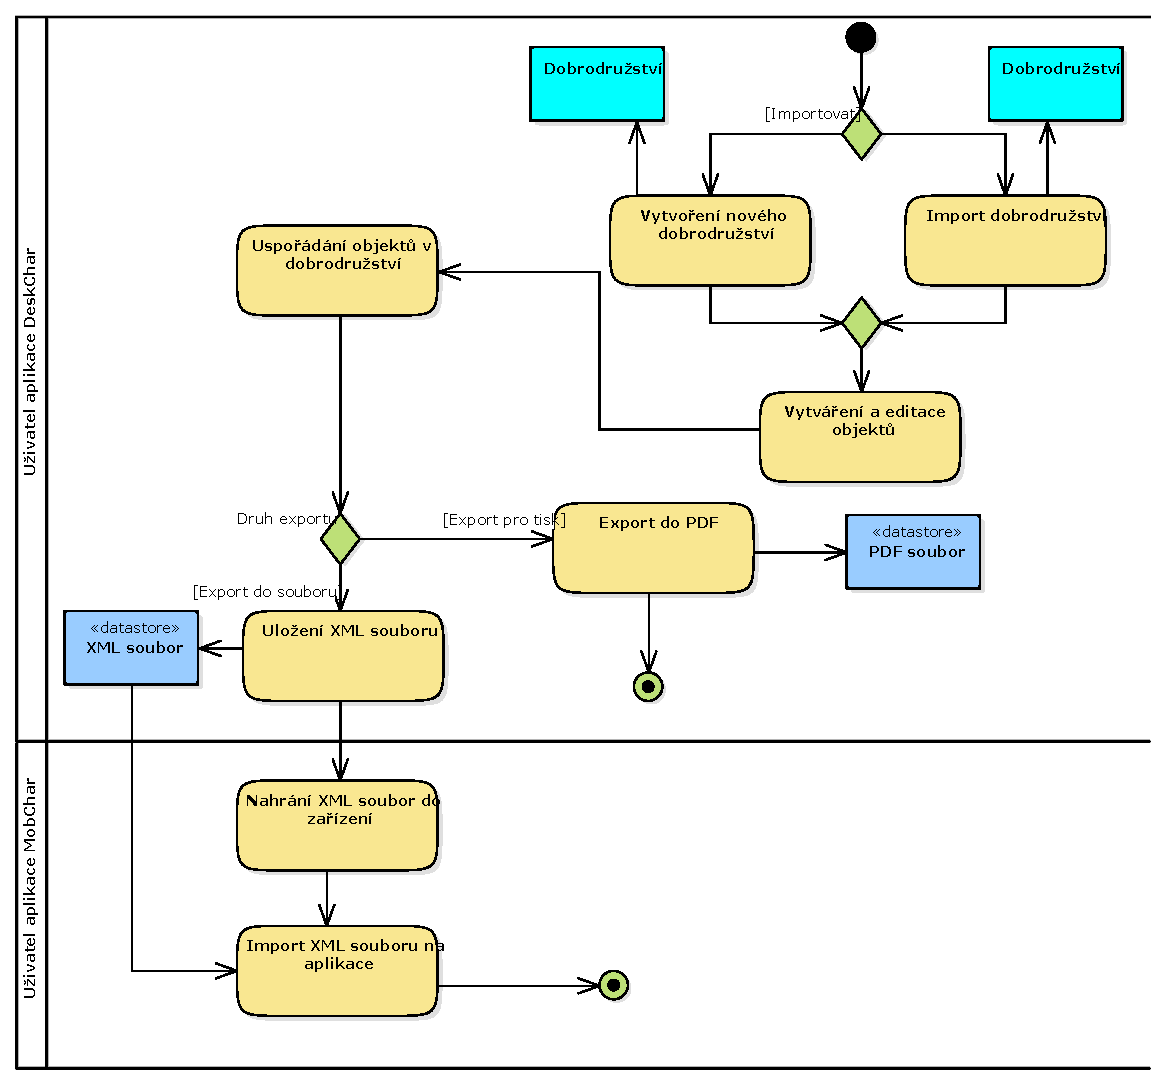
\includegraphics[width=0.8\textwidth]{images/business_dobrodruzstvi}
	\caption[Business proces vytváření dobrodružství]{Model bussines procesů vytváření dobrodružství}\label{fig:bp_dobrodruzsvi}
\end{figure}
Diagram \ref{fig:bp_dobrodruzsvi} popisuje proces, při kterém vzniká nové dobrodružství. Jak už jsem dříve zmiňoval, tak dobrodružství je také šablona. Protože se jedná o hlavní šablonu, která v sobě obsahuje větší počet šablon různých druhů, rozhodl jsem se vytváření dobrodružství popsat více do podrobna. Na začátku procesu vytvoříme nové dobrodružství nebo importujeme již existující a dále budeme upravovat již stávající hodnoty. V bodě \textbf{Vytváření a editace objektů} se jedná o businnes proces popsaný v kapitole \ref{sec:vytvareni_sablon},ve kterém vytvoříme veškeré potřebné objekty, které budou součástí dobrodružství. Do dobrodružství veškeré šablony přidáme a rozřadíme podle potřeby ( podle částí dobrodružství, podle typu šablony atd.). Když máme veškeré úpravy hotové, můžeme výsledné dobrodružství exportovat. Zde si můžeme vybrat zda budeme exportovat dobrodružství pro tisk do formátu PDF nebo pro MobChar ve formátu XML.\\
\textbf{Formát pro tisk:} Vybereme části, které chceme exportovat (nemusíme exportovat celé dobrodružství naráz) a provedeme export. Vytvoří se nám přehledný PDF soubor který následně můžeme vytisknout nebo nahrát do zařízení, které umí pracovat s formátem PDF.\\
\textbf{Formát pro MobChar:} Při exportu do formátu XML se vždy exportuje celé dobrodružství. Nedají se vybrat pouze některé části. Aplikace vytvoří XML soubor. Uživatel následně získaný soubor nahraje do zařízení a importuje ho do aplikace. Takto vytvořené dobrodružství je určené pro MobChar rozšíření pro pána jeskyně.

	\section{Doménový model}
Doménový model má za úkol popsat strukturu tříd v aplikaci a jejich vazby mezi nimi. Pro zaznamenání se využívá UML diagram. Diagram nepopisuje jednotlivé funkce tříd ani proměnné, které slouží k implementaci tříd, ale zachycuje pouze základní strukturu.
\subsection{Stromová struktura}
\begin{figure}\centering
	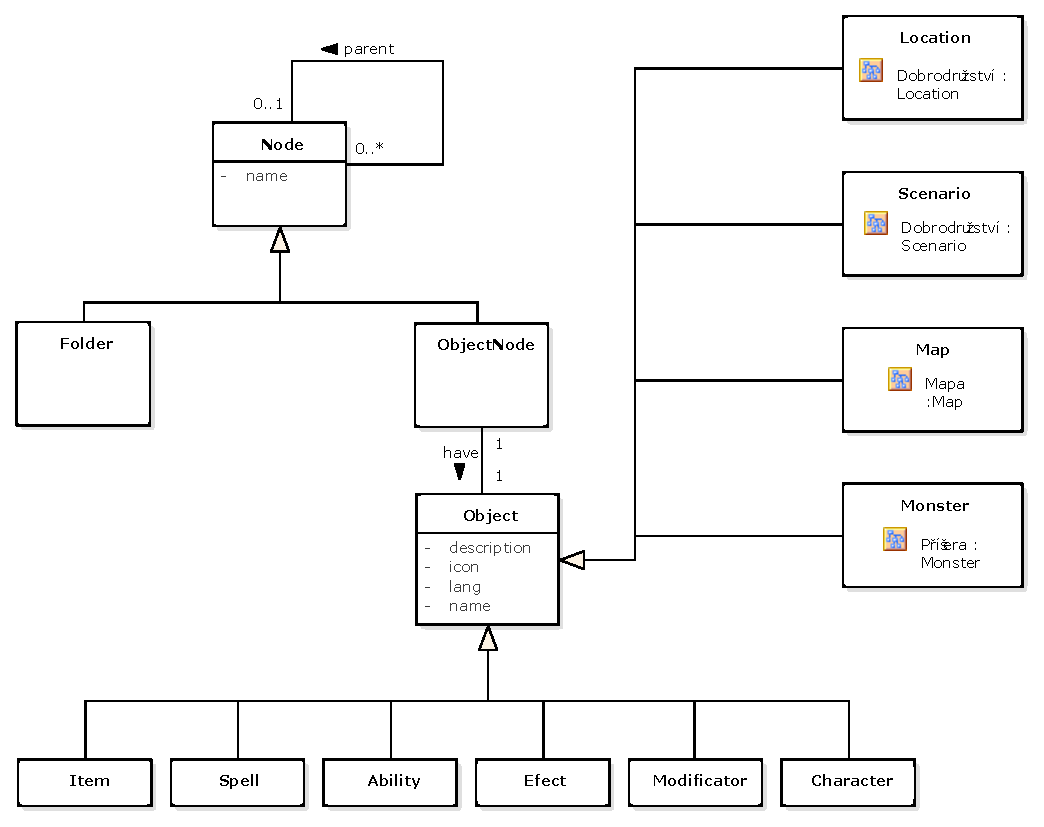
\includegraphics[width=0.8\textwidth]{images/domain_struktura}
	\caption[Analytický doménový model stromové struktury]{Analytický doménový model stromové struktury}\label{fig:dm_stromova_struktura}
\end{figure}
Diagram na obrázku \ref{fig:dm_stromova_struktura} popisuje strukturu objektů, které slouží pro uchování všech objektů (šablon) a jejich rozřazení do stromové struktury. Veškeré šablony využívají tuto stromovou strukturu. Třída Folder (složka) slouží pouze k rozřazování jednotlivých objektů do skupin. Složka má pouze jméno a může obsahovat libovolný počet složek nebo objektů. ObjektNode pak slouží k uchování šablony. Dolní část objektů (Item, Spell, atd.) jsou objekty, které jsou totožné s aplikací MobChar a slouží k uchování šablon pro základní aplikaci a využívají se i v aplikaci pro pána jeskyně. Pokud vás zajímá podrobnější popis těchto objektů, nahlédněte do bakalářské práce týkající se MobCharu. O proti tomu, objekty na pravé straně diagramu (Map item, Scenarion, atd.) jsou objekty, které slouží převážně k vytvoření dobrodružství. Jejich podrobnější popis naleznete dále.\\
\\
Veškeré objekty můžou mít potomky. Systém složek slouží pouze pro přehledné uspořádání. Každý objekt má definované objekty, které může mít jako potomky. Tento systém slouží pro ukládání závislostí, například dobrodružství může obsahovat mnoho lokací, příšer, map. Některé objekty, jako například kouzla a schopnosti, žádné potomky mít nesmějí. 
\subsection{Dobrodružství}
\begin{figure}\centering
	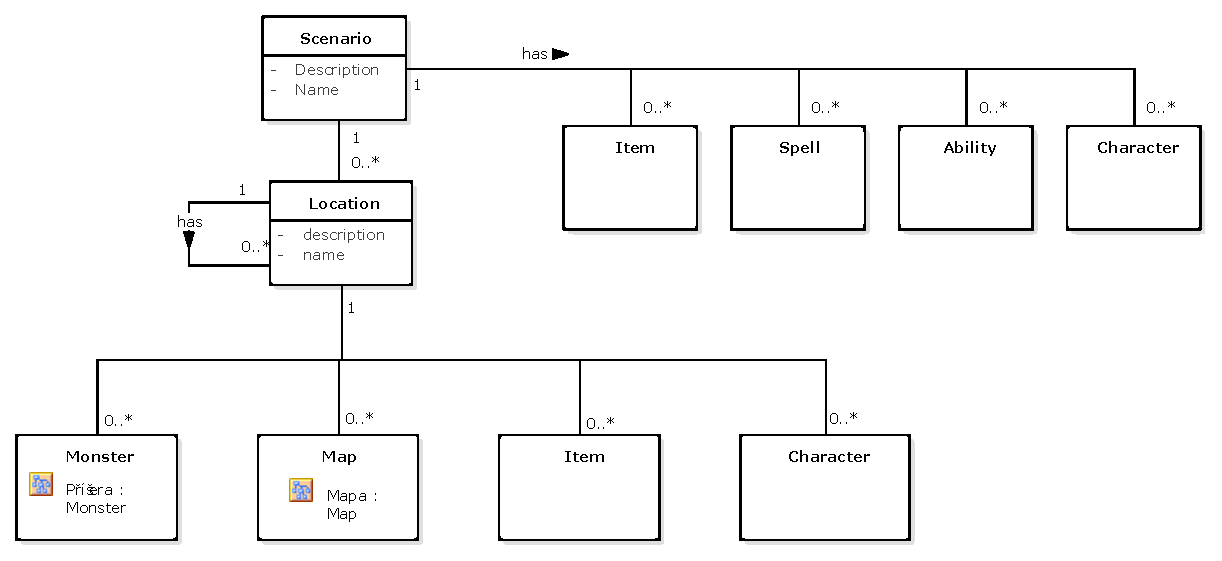
\includegraphics[width=0.8\textwidth]{images/domain_scenario}
	\caption[Analytický doménový model dobrodružství]{Analytický doménový model dobrodružství}\label{fig:dm_scenario}
\end{figure}
Diagram na obrázku \ref{fig:dm_scenario} popisuje strukturu pro ukládání a práci s dobrodružstvím. Hlavní třída scenario je rozdělená do jednotlivých lokací. Pro celé dobrodružství jsou však společné předměty, kouzla, schopnosti a postavy. Předměty, kouzla a schopnosti jsou pro pána jeskyně, který je nadále poskytuje hráčům, například pokud se hráč má možnost naučit nové kouzlo, nebo získal důležitý předmět pro dobrodružství (elixír, mapa, atd.). Třída Character zde zastupuje postavy hráčů, kteří dané dobrodružství hrají. Jedná se o stejné třídy jako v původní aplikaci MobChar. Pro přesnější popis těchto tříd, nahlédněte do bakalářské práce aplikace MobChar.\\
\\
Celé dobrodružství je členěné do lokací, které se navíc můžou do sebe zanořovat (lokace může mít pod sebou další lokace). Lokace obsahují příšery, mapy, předměty a postavy. Příšery mají velice podobnou strukturu jako postavy, můžou se naučit schopnosti a kouzla a vlastnit předměty, mají však odlišné atributy, proto jsou od postav odděleny. Jednotlivé mapy mají složitější strukturu, která je popsána níže. Předměty zde znamenají, předměty důležité pro tuto lokaci (klíče, věci v bednách a další). Poslední částí jsou postavy, které zde znázorňují postavy, za které nehrají hráči, ale samotný PJ. Jsou to důležité postavy pro dobrodružství, které se nacházejí v dané lokaci. Objekt je stejný jako klasické postavy, ale význam je trochu odlišný.
	\section{Model architektury}
\begin{figure}\centering
	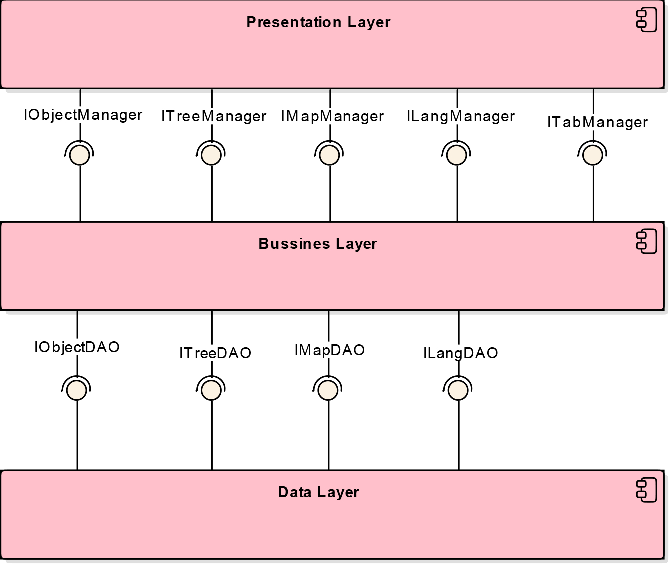
\includegraphics[width=0.8\textwidth]{images/architektura}
	\caption[Model architektury]{Model architektury}\label{fig:architektura}
\end{figure}
Model architektury popisuje formální popis systému případně jeho detailní plán na úrovni komponent vedoucí k jeho implementaci.\\
\\
Zvolil jsem třívrstvou architekturu z důvodu dobré přehlednosti a jednoduchém nahrazení jedné z části, bez zásahu do ostatních vrstev. Veškeré vrstvy mezi sebou komunikují na základe definovaného rozhraní.\\
\subsection{Vrstvy}
\textbf{Prezentační vrstva} zobrazuje informace pro uživatele. Jedná se o grafickou část celé aplikace. Kontroluje zadané vstupy, nijak však získané data nezpracovává.\\
\textbf{Business vrstva} je základní logická část aplikace. Leží zde jádro aplikace, její logika a funkce pro zpracování dat.\\
\textbf{Datová vrstva} je vrstva, která se stará o práci s daty. Zajišťuje komunikaci s databází a práci s XML soubory. Jejím základním úkolem je získat data z databáze nebo XML a převést je na objekty. \\
\subsection{Rozhraní}
Mezi vrstvami jsou definovaná rozhraní, které je nutné dodržet. Rozhraní začínají velkým písmenem I, konkrétní implementace daného rozhraní obvykle má stejný název, pouze bez počátečního písmena I.\\
\\
\textbf{IObjectDAO} je skupina několik DAO tříd, které se starají o přístup k datům z databáze a z XML. Na diagramu \ref{fig:architektura} je zobrazen pouze zástupný IObjectDAO, který v implementaci neexistuje a je nahrazen všemi DAO třídami (ISpellDAO, IEffectDAO atd.).\\
\textbf{ITreeDAO} se stará o~veškeré ukládání stromové struktury do databáze. \\
\textbf{IMapDAO} se stará o ukládání veškerých dat, které se týkají map. Rozhraní je společné pro všechny druhy map (grafické, jednoduché, obrázkové)\\
\textbf{ILangDAO} se stará o ukládání jazyků, které jsou v aplikaci použity. Nejedné se o překlady prezentační vrstvy, ale o jazyky vytvořené pro překlady šablon. Rozhraní se nestará o ukládání samotných překladů, pouze o jejich jazyky.\\
\\
\textbf{IObjectManager} navazuje na IObjectDAO. Jedná se opět o skupinu tříd pro veškeré základní objekty (ISpellManager, IAbilityManager, atd.). Rozhraní definuje jak přijímá data z prezentační vrstvy. Základní funkcionalita spočívá ve zpracování dat z prezentační vrstvy a vytvoření kompletního objektu, se kterým se dále pracuje nebo pošle na datovou vrstvu pro uložení.\\
\textbf{ITreeManager} se stará u připravení stromové struktury pro zobrazení. Vytváří z objektů stromovou strukturu a přidává do struktury metadata, které slouží pro zobrazení a práci na prezentační vrstvě.\\
\textbf{IMapManager} se stará o zpracování dat ohledně mapy. Převádí zobrazenou mapu pro uživatele na formu, ve které se dá snadno uložit do databáze. Propojuje veškeré šablony s mapou.\\
\textbf{ILangManager} se stará o zpracování dat z prezentační vrstvy ohledně jazyků.\\
\textbf{ITabManager} se stará o vytváření překladových záložek pro prezentační vrstvu. Toto rozhraní nemá DAO rozhraní, protože veškeré informace které potřebuje, získá přímo z konkrétních IObjectDAO tříd. Jejím hlavním úkolem je zpracování všech překladů jedné šablony a připravení objektů pro uložení.\\


\chapter{Návrh}
	\section{Model databáze}
	\begin{figure}\centering
	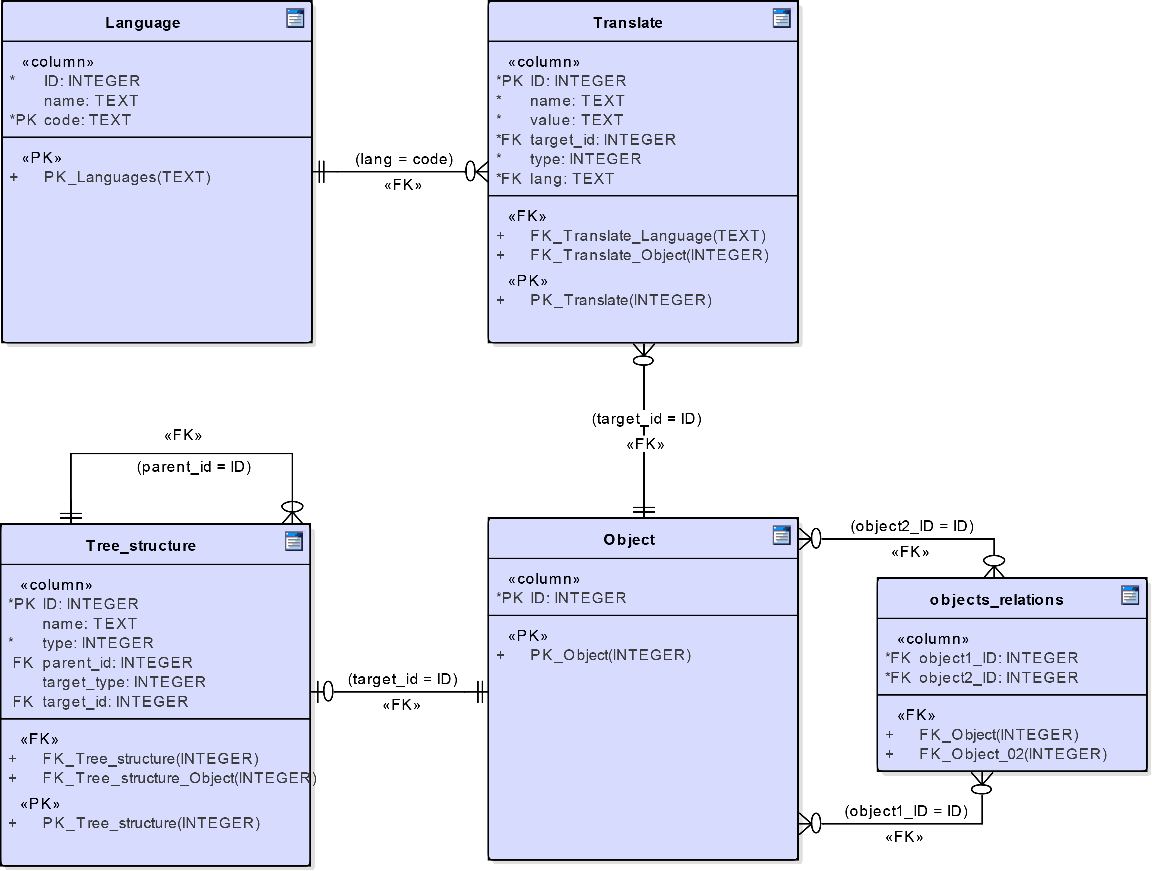
\includegraphics[width=0.8\textwidth]{images/database_basic}
	\caption[Základní model databáze]{Základní mode databáze}\label{fig:db_basic}
	\end{figure}
	Pro realizaci aplikace DeskChar jsem vybral databázi sqlite, která je jednoduchá a nepotřebuje žádný složitý externí software pro běh. Na druhou stranu zvládá veškeré potřebné operace, jako jsou cizí klíče a kaskádové mazání záznamů. Pro vytváření a práci se stromovou strukturou, je kaskádové mazání nedocenitelný pomocník. \\
\\
Diagram na obrázku \ref{fig:db_basic} je zjednodušený pro větší přehlednost. Na diagramu je zachycena základní struktura a princip závislostí v~databázi. Kompletní model databáze se nachází v~příloze.\\
\\
Z důvodu vícejazyčnosti šablon, bylo zapotřebí navrhnout strukturu databáze, která dokáže uložit neomezený počet jazykových překladů. Na obrázku \ref{fig:db_basic} můžeme vidět základní strukturu databáze. Tabulka Languages obsahuje záznamy o jazycích. Údaj o~jazyku není pouze textový v tabulce Translate, abychom docílili konzistence mezi záznamy pro stejný jazyk. Primárním klíče každého jazyka je textový kód, který je unikátní. V tabulce Translate pak nalezneme veškeré textové řetězce, které se nacházejí v objektech. Jeden záznam tabulky translate je přiřazen ke konkrétnímu objektu pomocí dvojice klíčů target\_type, který určuje o jaký objekt (tabulku v databázi) se jedná, a target\_id, který určuje konkrétní záznam v tabulce (ukazuje na primární klíč ID v tabulce). Informace o překladu jsou uloženy ve dvojici klíčů name a vulue, které slouží jako slovník, jejich jazyk určuje záznam lang. Takto zvolený návrh databáze umožňuje neomezený počet jazyků a jednoduchou rozšířitelnost.\\
\\
Druhá část diagramu se týká stromové struktury, která se používá pro všechny objekty v aplikaci. Tabulka Tree\_structure slouží pro zaznamenávání stromové struktury pro veškeré objekty. Do tabulky se ukládají dva druhy uzlů, složky a objekty. Atribut type určuje, o který druh uzlu se jedná. Pomocí cizího klíče parent\_id, vzniká stromová struktura. Zde se využívá kaskádové mazání, pokud se smaže záznam, který má pod sebou navázané další záznamy pomocí cizího klíče, smažou se tyto záznamy také automaticky v databázi. Tento princip udržuje tabulku konzistentní a nevznikají žádné záznamy, které se již nepoužívají. Každý uzel který je typu object, ukazuje pomocí dvojice klíčů target\_type, který určuje tabulku v databázi, a target\_id na záznam v ostatních tabulkách. V diagramu je to naznačené zjednodušeně, kde tabulka Object zastupuje tabulky všech objektů (Spell, Item, atd.). \\
\\
Poslední část diagramu znázorňuje, jak jsou vyřešené vztahy mezi objekty. V databázi je zapotřebí zachytit mnoho vazeb mezi objekty. Protože se jedná o systém šablon, kde jedna šablona můžu patřit k více objektům a tato situace bude nastávat velmi často, rozhodl jsem se záznamy nekopírovat pro každý objekt, ale použít systém odkazů. Tyto odkazy realizují tabulky v diagramu znázorněné jako objects\_relations. Jedná se o jednoduché tabulky, které obsahují pouze dva cizí klíče, jeden ukazující na záznam rodiče a druhý ukazující na záznam přiřazené šablony. Tyto tabulky se jmenují podle objektů které spojují, rodičovský objekt je první a názvy jsou oddělené čárkami.
	\section{Model komunikace}
	\begin{figure}\centering
	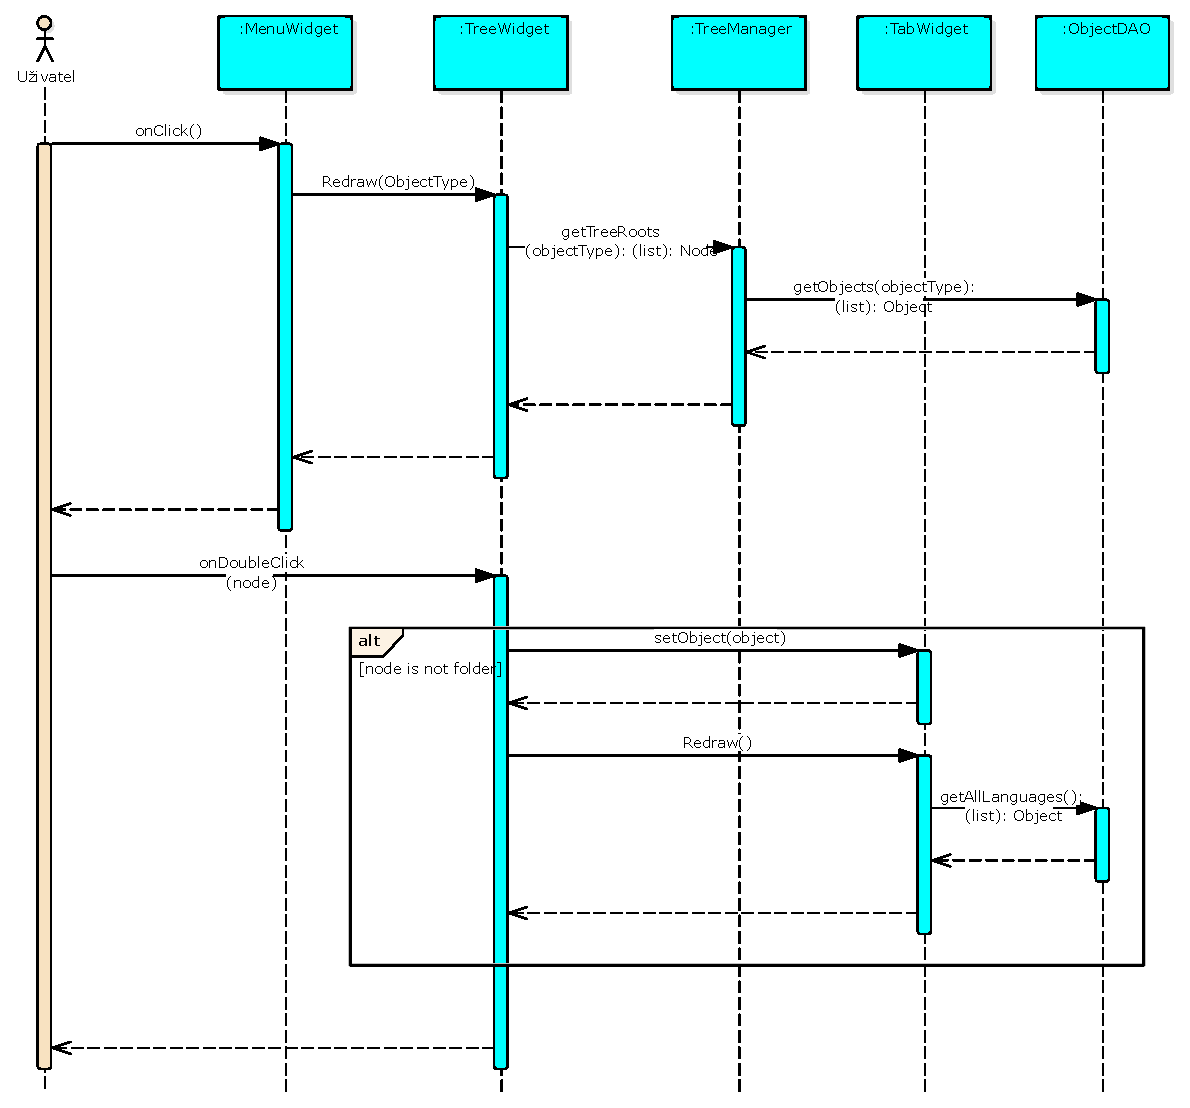
\includegraphics[width=0.8\textwidth]{images/comunication_main}
	\caption[Model komunikace pro hlavní obrazovku]{Model komunikace pro hlavní obrazovku}\label{fig:comunication_main}
	\end{figure}
Nejčastější operaci prezentační vrstvy, což je práce se stromovou strukturou a vytváření překladů, jsem vytvořil diagram komunikace, který znázorňuje komunikaci mezi jednotlivými třídami. Na diagramu \ref{fig:comunication_main} můžeme vidět základní dvě činnosti. Vybrání konkrétního typu šablon a zobrazení stromové struktury a zobrazení hlavního widgetu pro vytváření šablon po vybrání konkrétní položky ve stromové struktuře.\\
\\
Uživatel v menu klikne na požadovaný druh šablon. Tím se zavolá funkce Redraw, která má na starosti vykreslení stromové struktury ve widgetu. Potřebná data získá z TreeManageru po zavolání funkce getTreeRoots, která má na starosti, vytvoření kompletního stromu uzlů, přičemž vrací seznam kořenových uzlů. TreeWidget z tohoto listu pomocí rekurze vykreslí celý strom. TreeManager získává data z konkrétní DAO třída (v diagramu zjednodušena jako ObjectDAO). Objekty navěšené na uzly stromu můžou být různé, takže třída TreeManager volá více DAO tříd.\\
\\
Druhá část diagramu se týká vykreslení hlavní části obrazovky, kde se vytváří samotné šablony a jejich překlady. Uživatel v TreeWidgetu dvakrát klikne na nějaký uzel. Pokud se jedná o objekt zavolá se nad třídou TabWidget funkce Redwar, která s parametrem object type. Object type určuje, na který objekt bylo v TreeWidgetu kliknuto, podle kterého se zavolá znovu konkrétní DAO třída pro daný objekt. Třída vrátí seznam objektů, přičemž se jedná o jednu šablonu, ale ve všech jazycích, ve kterých byla vytvořena. TabWidget následně pro každý jazyk vykreslí jednu záložku, kde se dají hodnoty šablony upravovat nebo případně vytvořit nový překlad pro nový jazyk.
	
	\section{Model nasazení}
	\begin{figure}\centering
	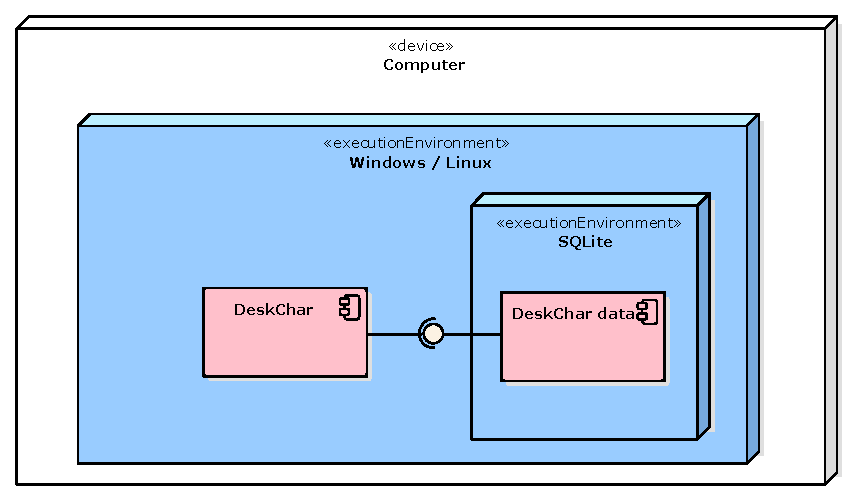
\includegraphics[width=0.8\textwidth]{images/model_nasazeni}
	\caption[Model nasazení]{Model nasazení}\label{fig:model_nasazeni}
	\end{figure}
Diagram nasazení zobrazuje způsob rozdělení systému na samostatné části a komunikační vazby mezi nimi, čímž definuje architekturu systému. Nalezneme zde veškeré komponenty systému a všechny potřebné části pro běh našeho systému.\\
\\
Na diagramu \ref{fig:architektura} můžeme vidět, že software je určený pro počítače a funkční pod operačními systémy Windows a Linux (verze operačního systému jsou uvedeny v sekci nefunkční požadavky). Aplikace je napsaná v pythonu a zabalená do spustitelného balíčku, který nevyžaduje žádné speciální požadavky na systém. Veškeré potřebné knihovny a prostředí má uložené v balíčku. Databáze sqlite běží v rámci tohoto balíčku také a nepotřebuje žádné dodatečné prostředí.

\chapter{Realizace}

\begin{conclusion}
	%sem napište závěr Vaší práce
\end{conclusion}

\bibliographystyle{csn690}
\bibliography{resources/mybibliographyfile}

\appendix

\chapter{Seznam použitých zkratek}
% \printglossaries
\begin{description}
	\item[HnH] Hra na hrdiny
	\item[DrD] Dračí doupě
	\item[RPG] Role-playing game
	\item[PJ] Pán jeskyně
	\item[DAO] Data access object
	\item[MobChar] Mobile character
	\item[DeskChar] Desktop character	
\end{description}

 

\chapter{Obsah přiloženého CD/USB}

%upravte podle skutecnosti

\begin{figure}
	\dirtree{%
		.1 readme.txt\DTcomment{stručný popis obsahu CD}.
		.1 exe\DTcomment{adresář se spustitelnou formou implementace}.
		.1 src.
		.2 impl\DTcomment{zdrojové kódy implementace}.
		.2 thesis\DTcomment{zdrojová forma práce ve formátu \LaTeX{}}.
		.1 text\DTcomment{text práce}.
		.2 thesis.pdf\DTcomment{text práce ve formátu PDF}.
		.2 thesis.ps\DTcomment{text práce ve formátu PS}.
	}
\end{figure}

\end{document}
